\cotefile{127}
\scanpage{14}
% archive sheet number: 13
% L1
Considérons p.ex. \deleted{\unsure{de}} le faisceau d'anneaux
% L2
\unsure{standard|standart|structural} $O$ sur $C$, et considérons un
% L3
module $\deleted{\unsure{A}}F$ \inserted{quasi-cohérent} sur $O$. \deleted{En \illegible{2} $\unsure{\mathcal E}, F_{\unsure{\mathcal E}}$}
% L4
\deleted{\illegible{2}} Alors $F$ induit sur chaque
% L5
% slanted
\margin{à vérifier}
$\mathcal M_{/T}$ (pour
\diagram{\begin{tikzcd}[ampersand replacement=\&,row sep=0.15em,column sep=small]
X \& \& {}\\
{} \& T_0\arrow[ul,"\unsure{h|h_0}"']\arrow[r] \& T
\end{tikzcd}}) un faisceau \uline{quasi-cohérent},
% L6
avec \unsure{contravariance|isomorphismes} en l'objet variable (\diagram{\begin{tikzcd}[ampersand replacement=\&,row sep=0.18em,column sep=small]
X \& {}\\
T_0\arrow[u]\arrow[r] \& T
\end{tikzcd}})
% L7
de $C$, et de façon \deleted{\illegible{1}}\uline{cartésienne} \ldots. \deleted{De plus,}
% L8
on voit que l'on obtient en particulier
% L9
un ``faisceau formel'' sur le
% L10
complété formel d'un \deleted{$X$ \unsure{du|de}} $Z$ le long de
% L11
$X$ [pour une \unsure{imm|imm.} $\delta\colon X\unsure{-|\to} Z$, dont
% L12
les voisinages \unsure{infin.} sont $\in\operatorname{Ob}\,\underline{\unsure{S|Z|\mathcal S|\mathcal C}}$] et on
% L13
obtient alors, par une vérification essentiellement
% L14
facile
% L15
% slanted
\margin{\unsure{préciser|précision} et à vérifier.}
\[
H^*(\unsure{e|C|\ell|\mathcal C}_{/\delta},F)\simeq H^*(\widehat Z,F\mid\widehat Z)
\]
% L16
où le deuxième \unsure{mb} est pris comme
% L17
cohomologie dans la catégorie des systèmes
% L18
projectifs adiques sur le complété formel
% L19
$\widehat Z$ de $Z$ le long de $X$ \ldots\,.

\scanpage{15}
% L1
\[
F\qquad F_U\longrightarrow G_U
\]
\diagram{\begin{tikzcd}[ampersand replacement=\&,column sep=small,row sep=small]
F\arrow[r]\arrow[d] \& i_*(G_U)\\
G\arrow[ur] \&
\end{tikzcd}}
% L2–4
\diagram{\begin{tikzcd}[ampersand replacement=\&,column sep=small,row sep=small]
X\supset U\arrow[dd,"f"'] \& \& \&\\
\& X'\arrow[d,dash]\arrow[r,phantom,"\unsure{\supset|\twoheadrightarrow}"] \& U'\arrow[dl,dash] \& G'\\
Y\arrow[r,dash] \& Y'\arrow[u,bend left=42] \& \substack{\widetilde{x}_1\\[-2pt]\vert\\[-2pt]\widetilde{x}} \& \widetilde{x}'
\end{tikzcd}}
% L3–5 right
\[
A=\varprojlim(A_\alpha=A/\unsure{J_{\alpha+1}|J^{\alpha+1}|I_{\alpha+1}|I^{\alpha+1}|\mathfrak J^{\alpha+1}})\qquad f
\]
\[
\left.\begin{aligned}M&\to{}N\\ M_{\alpha_f}&\xrightarrow{\sim}N_{\alpha_f}\end{aligned}\right|
\Longrightarrow
\left|\begin{aligned}&\forall p\in\operatorname{Spec} A,\\&f\notin p,\\&M_p\simeq N_p\\&(\text{car }\widehat M_p\simeq\widehat N_p)\end{aligned}\right.
\]
% L6 right
\diagram{\begin{tikzcd}[ampersand replacement=\&,row sep=0.3em]
A\arrow[r] \& B\\
\rotatebox{90}{$\subset$} \&\\
\unsure{\mathfrak R|\mathfrak r|\mathfrak A} \& \mathfrak R B
\end{tikzcd}}
\[
(\mathfrak R B\cap A)/\deleted{\mathfrak R}\mathfrak R
\]
% L6–10 left and centre
\[
\begin{aligned}
&\deleted{x_\alpha\in\operatorname{Ass}G_{\unsure{U|X}}}\\
&\deleted{(\Longrightarrow x_\alpha\in\operatorname{Ass}\underline{G_y})}\\
&\deleted{T_\alpha=\overline{\{x_\alpha\}}}
\end{aligned}
\]
\diagram{\begin{tikzcd}[ampersand replacement=\&,row sep=small,column sep=large]
\deleted{x'\in(T_\alpha)_{y'}}\arrow[dd]\arrow[d,dash,bend right=30] \& \text{EGA }\boxed{\mathrm{IV}}\ 12.2.\unsure{.|{}}\\
\text{\deleted{pt maximal}} \& \deleted{\Longrightarrow x'\in\operatorname{Ass}G_{y'}}\arrow[d,Rightarrow]\\
\deleted{y'} \& \deleted{x'\in U_{y'}}
\end{tikzcd}}
% L8–10 right
\[
\deleted{A/\mathfrak R\overset{?}{\hookrightarrow}B/\mathfrak R B}
\qquad A/\mathfrak R_\alpha\hookrightarrow \unsure{B/\alpha'|B\alpha'|B/\alpha|B_\alpha}
\]
\smallskip\hrule\smallskip
% L11–13
\diagram{\begin{tikzcd}[ampersand replacement=\&,row sep=small]
X\arrow[d,"\text{birationnel}"']\\Y
\end{tikzcd}}
\[
\begin{aligned}
&U=\inserted{\text{l'ouvert où } f\ \text{est }\simeq}\unsure{Y|V|\vert},\quad G=O_X,\quad T=X,\quad T_{y'}\ \text{de dim }0\\
&G'\unsure{\simeq|=}O_U,\hspace{9em}T_y\ \text{de dim }1
\end{aligned}
\]
\smallskip\hrule\smallskip
% L14–16 left
\figure{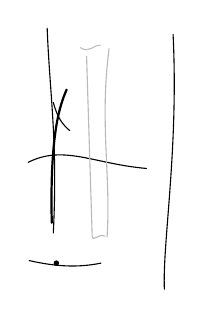
\begin{tikzpicture}[x=0.65cm,y=0.65cm,line cap=round]
\draw (0.6,5.1) .. controls (0.65,3.8) and (0.81,2.9) .. (0.72,1.1);
\draw[thick] (0.98,3.9) .. controls (0.85,3.6) and (0.65,3.05) .. (0.69,1.3);
\draw (0.72,3.65) .. controls (0.8,3.35) and (0.9,3.22) .. (1.04,3.1);
\draw (0.23,2.48) .. controls (0.92,2.83) and (1.51,2.45) .. (2.54,2.36);
\draw[gray!50] (1.25,4.72) .. controls (1.43,4.6) and (1.52,4.79) .. (1.64,4.77);
\draw[gray!55] (1.37,4.55) -- (1.48,1.03) .. controls (1.48,0.92) and (1.6,1.09) .. (1.73,1.04);
\draw[gray!55] (1.81,4.7) .. controls (1.62,3.25) and (1.85,2.2) .. (1.77,1.02);
\draw (0.25,0.56) .. controls (0.78,0.44) and (1.2,0.42) .. (1.65,0.51);
\fill (0.78,0.51) circle (1pt);
\draw (3.06,4.98) .. controls (3.17,2.75) and (2.85,0.88) .. (2.89,0);
\end{tikzpicture}}
% L14–16 centre and right
\diagram{\begin{tikzcd}[ampersand replacement=\&,row sep=small]
x_\alpha\in\operatorname{Ass}G_U\arrow[d,dash]\\ y
\end{tikzcd}}
\[
\begin{aligned}
T_\alpha&=\overline{\{x_\alpha\}}\\
(T_\alpha)_{y'}\cap U&\ \text{est dense ds }(T_\alpha)_{y'}
\end{aligned}
\]
% archive sheet number: 14

\scanpage{16}
% L1
Dém. de 1.5.

% L2
\margin{1.4.2}\uline{Remarque 1} \quad les conditions b), c) de 1.4 $\Longleftrightarrow$ après
% L3
$\forall$ \unsure{changt|chgt} de base $S'\unsure{-|\to}S$, $S'$ artinien,
% L4
$\exists$ solution

% L5
\margin{1.4.3}\uline{Remarque 2} \quad a) $\Longleftarrow$ $\exists$ solution après $\forall$ chgt. de
% L6
base $S'\mathrel{-}S$, $S'$ trait

% L7
\uline{Vrai théorème}\quad 1.4
% L8
\margin{\uline{Énoncé} \uline{final}}\uline{Corollaire}\quad $\exists$ solution $\Longleftrightarrow$ $\exists$ solution après tt
% L9
chgt. de base $S'\mathrel{-}S$,
% L10
$S'\left\{\begin{aligned}&\text{artinien}\\&\text{\uuline{trait}}\end{aligned}\right.$
\margin{inutile si les $\widehat{\underline O}_{\unsure{Y,y|y,y}}$ réduits}

% L12
\deleted{Pour prouver 1.5, il suffit donc de prouver
% L13
qu'après $S'\mathrel{-}S$, $S'$ trait, $\exists$ solution. Donc
% L14
$OPS$ $S$ est un trait.}

% L15–17 left
\diagram{\begin{tikzcd}[ampersand replacement=\&,column sep=small,row sep=small]
\deleted{F=G} \& \deleted{G_U}\\
\deleted{X}\arrow[r,phantom,"\deleted{\unsure{\supset|-}}"]\arrow[d] \& \deleted{U}\\
\deleted{S} \&
\end{tikzcd}}
% L15–17 right
\deleted{$F=\unsure{C|G}$ est plat /$S$. Alors $\forall x\in\operatorname{Ass} G_U$,
$x'\in\text{Maximal de }(T=\overline{\{x\}})_y\Longrightarrow x'\in\operatorname{Ass}G_y$
donc}

% L18
\diagram{\begin{tikzcd}[ampersand replacement=\&,row sep=small]
x\in\operatorname{Ass}G_U\arrow[d,dash]\\ y'
\end{tikzcd}}
% L18–19
\[
T=\overline{\{x\}}\qquad y\in Y\qquad T_y\ne\varnothing.
\]
% L19–22
les comp de $T_y$ sont de dim $\geq(T_{y'})=d$
donc ce sont des composantes des $X_y$.
% archive sheet number: 15

\scanpage{17}
% L1
\uline{Lemme} 1.4.1 : Les notations et les hypothèses étant
% L2
\unsure{celle|celles} de (1.1) supposons que $X$ et $Y$ soient localement
% L3
noethériens et $G=\operatorname{Im}(F\longrightarrow i_*(G_U))$ cohérent. Soient
% L4
\deleted{$Z$ le sous-schéma \inserted{réduit} de $X$ ayant $X-U$ comme espace
% L5
sous-jacent} $Z=X-U$ et $y\in f(Z)$ \deleted{tel que}
% L6
\textcircled{d} $\forall x\in Z_y=X_y\cap Z$ l'anneau local $\underline O_{X,x}$ soit à fibres formelles
% L7
géométriquement normales

% L8
On Suppos\deleted{\unsure{ons}}\textcircled{a} $\forall x'\in\operatorname{Ass}(G_U)$ posant $T=\overline{\{x'\}}$ alors
% L9
$T_y\cap U$ est dense dans $T_y$ et que la même condition
% L10
soit vraie sur tout $X'$ étale sur $X$

% L11
\deleted{\unsure{S}}\textcircled{b} il existe une famille de
% L12
morphismes locaux $Y_i\longrightarrow Y'=\operatorname{Spec}\widehat{\underline O}_{Y,y}$
% L13
tels qu'après chacun des changements de
% L14
base $Y_i\longrightarrow Y$ le problème ait une solution
% L15
et que l'intersection des noyaux des homomorphismes
% L16
canoniques $\widehat O_{Y,\unsure{y|g}}\longrightarrow\Gamma(Y_i,O_{Y_i})$ soit
% L17
réduite à $0$

% L18
\textcircled{c} Ou bien $f\colon X\longrightarrow Y$ est localement
% L19
de présentation \unsure{fini|finie} ou bien les $Y_i\longrightarrow Y'$
% L20
sont finis

% L21
Alors $\mathbf X$ est plat sur $\unsure{\mathbf y|\mathbf Y}$ en tout point de $X_y$
% L22
et $U_y$ contient $\operatorname{Ass}(G_y)$

% L23
En particulier si les conditions \deleted{\unsure{a}} précédentes
% L24
sont vraies en tout point $y$ de $f(Z)$ alors le
% L25
problème admet une solution cohérente.

% L26
\deleted{\illegible{1}}
% archive sheet number: 16

\scanpage{18}
% L1
expliciter les $H^{\unsure{q|n}}(C_{/\delta_i},F)$. Pour simplifier
% L2
la notation, on laisse tomber
% L3
l'indice $i$. \deleted{Notons que on} \inserted{Supposons}
% L4
\deleted{peut se \unsure{borner|besoins}}
% L5
que $\delta\in\mathcal N$ [i.e. $Z\in\operatorname{Ob}\,\underline{\unsure{S|\mathcal S|\mathfrak S}}$],
% L6
\deleted{donc} D'après un énoncé

% L3–6 left
\diagram{\begin{tikzcd}[ampersand replacement=\&,column sep=large,row sep=small]
X\arrow[r,"\delta"] \& Z.\\
T_0\arrow[u,"\varphi"]\arrow[r,"i"'] \& T\arrow[u,"u"']\\
T_0^{(i)}\arrow[u]\arrow[r] \& T^{(i)}\arrow[u,"u_i", "{\in\mathcal M}"'{draw,rounded corners=6pt,inner sep=1pt}]
\end{tikzcd}}
% L7
\unsure{standard|standart}, on peut remplacer $C_{/\delta}$ par
% L8
$(\mathcal M_{\unsure{C|0|{}}})_{/\delta}$, i.e. la catégorie des
% L9
diagrammes
\diagram{\begin{tikzcd}[ampersand replacement=\&,row sep=small,column sep=small]
X\arrow[r] \& Z\\
T_0\arrow[u,dash]\arrow[r,dash] \& T\arrow[u]
\end{tikzcd}}
qui sont des
% L10
\uline{morphismes \inserted{$\mathcal M$-}cartésiens} dans $C$, or cette
% L11
catégorie est \unsure{isomorphe|équivalente} à $\mathcal M_{/Z}$, avec
% L12
la topologie \unsure{héritée|héritie|induite} de $\unsure{\mathcal R|\mathcal T|\mathcal C}$. On trouve
% L13
donc
\[
H^q(C_{/\delta_i},F)\simeq H^q_{\mathcal M,\mathcal R}(\deleted{\unsure{X}}Z_n,F)
\]
% L14
et finalement
% L15
\[
\resizebox{.98\linewidth}{!}{$\displaystyle\boxed{0\longrightarrow\varprojlim\nolimits_n^{(1)}H^{\unsure{q|q-1}}_{(\mathcal M,\mathcal R)}(X_n^{(i)},F)
\longrightarrow H^q(X^{(i)},F)
\unsure{-|\to}\varprojlim\nolimits_n H^q_{(\mathcal M,\unsure{\mathcal T|\mathcal R|\mathcal C})}
\deleted{\unsure{(X_n}}(X_n^{(i)},F)\longrightarrow 0}$}
\]
% L16
[Sous l'hypothèse que les $X_n^{(i)}\in\operatorname{Ob}\,\underline S$]
% archive sheet number: 17

\scanpage{19}
% L1–5 left
\diagram{\begin{tikzcd}[ampersand replacement=\&,row sep=0.4em,column sep=small]
Z_U\arrow[ddr,dash,bend right=25,"\text{plat}"'] \& \& Z?\arrow[ll,phantom,"{\unsure{\longleftarrow|\lhook\joinrel\relbar|\hookrightarrow}}" description]\\
U\arrow[u,phantom,"\cap"] \& \subset \& X\arrow[u,phantom,"\cap"]\arrow[dl,dash]\\
\& Y \&
\end{tikzcd}}
% L1
$Z_U=Z\cap U$ et tel que $Z_U$ soit universellement /$Y$
% L2
sch. dense dans $Z$

% L3
NB si $Z$ \unsure{de|est} \inserted{loc. de} prés finie sur $Y$, ou $Y,Z$ noeth
% L4
alors \deleted{l'hyp \unsure{d'exig}} la condition envisagée
% L5
\[
\Longleftrightarrow\quad\forall y\in Y,\quad
\underset{\substack{\cap\\Z_y}}{Z_y\cap U}\supset\operatorname{Ass}Z_y
\]
\margin{EGA \uline{IV} 11.12.\textsuperscript{?}}
% archive sheet number: 18

\scanpage{20}
% L1–3
\diagram{\begin{tikzcd}[ampersand replacement=\&,row sep=small,column sep=small,execute at end picture={\draw[thin,rounded corners=12pt] ([xshift=-3pt]upperu.north west) -- ([xshift=-4pt]baseone.south west) -- (basetwo.south east) -- ([xshift=4pt]doubleu.east) -- ([xshift=5pt]sheaves.north east);}]
U \& |[alias=upperu]| U' \& |[alias=sheaves]| F'_{U'}\to\unsure{G_{U'}|G'_U|G'_{U'}} \& {}\\
X\arrow[r,dash]\arrow[d,dash] \& X'\arrow[d,dash] \ {\scriptstyle F'} \& X''\arrow[d,dash] \& |[alias=doubleu]| U'' \& F''_{U''}\to G''_{U''}\\
Y \& |[alias=baseone]| Y'\arrow[l,"\mathrm{fpqc}"'] \& |[alias=basetwo]| Y''\arrow[l,shift left=1.4]\arrow[l,shift right=1.4] \& Y'''\arrow[l,dash]\arrow[l,dash,shift left=2]\arrow[l,dash,shift right=2]
\end{tikzcd}}
% L4–7 left
\diagram{\begin{tikzcd}[ampersand replacement=\&,row sep=small,column sep=small]
U \& U' \& G'_{U'}\leftarrow F'\\
\& X'\arrow[dl,"\mathrm{fpqc}"']\arrow[ddl,bend left=60]\quad F' \&\\
X\arrow[d] \& F \&\\
Y \& \&
\end{tikzcd}}
% L4–6 right
pour tt $n$
\[
\begin{aligned}
&\exists J\unsure{\in|=}\{i_1\unsure{-|,\ldots,}i_{\unsure{r|n}}\}\subset I\\
&\unsure{\mathfrak R|\mathfrak r|\mathfrak A}_n\subset\operatorname{Ker}
\left(\underbrace{\widehat O_{Y,y}}_{A}\to\prod_{\alpha\in J}\underline O_{Y_{i_\alpha},y_{i_\alpha}}\right)
\subset\tikz[baseline=(power.base)]\node[draw,rounded corners=8pt,inner sep=2pt](power){$\widehat m_y^{\,n}$};
\end{aligned}
\]
% L6 right
OPS les $Y_i$ artiniens
% L7 right
\diagram{\begin{tikzcd}[ampersand replacement=\&,column sep=small,row sep=small]
{} \& A\arrow[r] \& \underline{A/\mathfrak R_n}\arrow[r,hook] \& \prod\underline O_{Y_\alpha,y_\alpha}\\
Z'_{\deleted{\unsure{\alpha}}}\quad Z'_i \&
\left\{\begin{gathered}Z'_i\cap U'_y\ne\varnothing\\
\text{i.e. }Z'_i\cap X'_y\ne\{x'\}\end{gathered}\right.\arrow[urr,bend right=23] \& \& {}
\end{tikzcd}}
% L9–11
\diagram{\begin{tikzcd}[ampersand replacement=\&,row sep=small,column sep=small]
G_{U'} \& U'\subset \& X'=X^{h}\arrow[d] \& X'_y\arrow[d]\supset U'_y\\
G_U \& U\subset \& X \& X_y\supset U_y\\
\& Z_{\unsure{\alpha_1|a_1|\alpha}} \& \&
\end{tikzcd}}
% L12–13 lower sketches
\figure{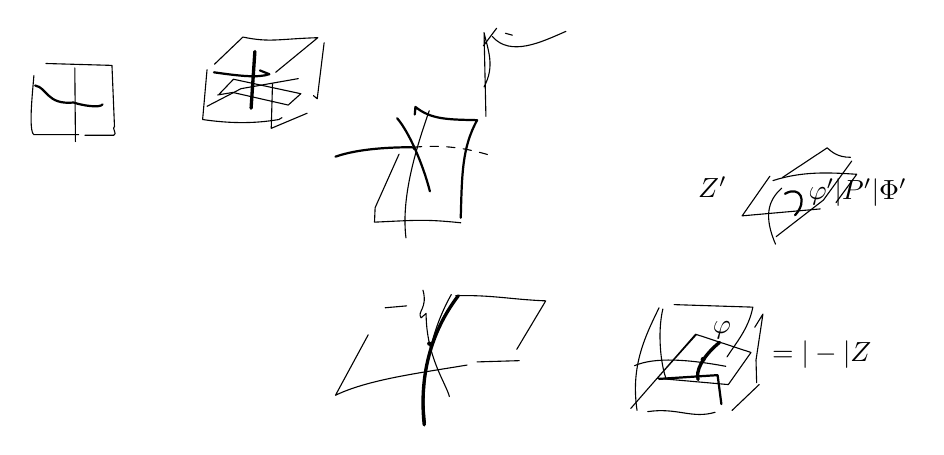
\begin{tikzpicture}[x=.008cm,y=-.008cm,line cap=round,line join=round]
\draw (244,1269) -- (349,1272) -- (353,1369) .. controls (348,1371) and (358,1381) .. (352,1383) -- (306,1383);
\draw (296,1382) -- (225,1382) .. controls (216,1376) and (223,1314) .. (225,1288);
\draw (290,1276) -- (291,1393);
\draw[thick] (227,1304) .. controls (246,1307) and (245,1335) .. (288,1331) .. controls (303,1336) and (330,1340) .. (334,1334);
\draw (512,1270) -- (557,1227) .. controls (600,1236) and (613,1230) .. (676,1228) -- (609,1283);
\draw (686,1236) -- (675,1325) -- (669,1320);
\draw (500,1279) -- (493,1358) .. controls (534,1364) and (573,1365) .. (614,1358) -- (619,1355);
\draw (604,1301) -- (602,1372) -- (659,1348);
\draw[thick] (511,1283) .. controls (553,1289) and (581,1292) .. (599,1286) -- (584,1280);
\draw[very thick] (576,1250) -- (570,1340);
\draw (500,1337) -- (554,1309) -- (645,1293);
\draw (519,1318) -- (542,1294) -- (649,1317) -- (629,1335) -- (541,1315) -- (517,1319);
\draw[thick] (704,1417) .. controls (741,1404) and (793,1402) .. (826,1402);
\draw[dashed] (828,1402) .. controls (885,1397) and (921,1406) .. (957,1417);
\draw (805,1413) -- (767,1498) -- (766,1521) .. controls (832,1518) and (845,1516) .. (903,1522);
\draw[thick] (903,1514) .. controls (905,1444) and (905,1403) .. (929,1359) .. controls (882,1358) and (856,1358) .. (831,1338) -- (830,1350);
\draw (853,1344) .. controls (826,1420) and (809,1489) .. (816,1546);
\draw[thick] (802,1356) .. controls (821,1378) and (843,1429) .. (854,1472);
\fill (829,1404) circle[radius=.024cm];
\draw (943,1353) -- (940,1220) .. controls (946,1247) and (958,1273) .. (940,1306);
\draw (939,1241) -- (960,1213);
\draw (953,1226) .. controls (982,1259) and (1031,1235) .. (1070,1218);
\draw (974,1221) -- (985,1224);
\node at (1303,1465) {$Z'$};
\draw (1394,1448) -- (1350,1511) -- (1474,1500);
\draw (1399,1455) .. controls (1445,1440) and (1488,1442) .. (1532,1445) -- (1499,1490);
\draw (1414,1450) -- (1485,1403) .. controls (1492,1409) and (1501,1418) .. (1522,1418);
\draw (1524,1424) -- (1479,1486) -- (1404,1544);
\draw (1413,1467) .. controls (1391,1486) and (1384,1512) .. (1403,1556);
\draw[thick] (1418,1476) .. controls (1442,1462) and (1455,1487) .. (1434,1510);
\node[right] at (1440,1474) {$\unsure{\varphi'|P'|\Phi'}$};
\draw (783,1657) -- (817,1654);
\draw (756,1700) -- (704,1796) .. controls (756,1771) and (835,1761) .. (913,1748);
\draw (929,1743) -- (996,1741);
\draw (992,1723) -- (1038,1646) .. controls (984,1644) and (950,1636) .. (895,1638);
\draw[very thick] (899,1638) .. controls (854,1697) and (837,1768) .. (845,1843);
\draw (888,1636) .. controls (849,1705) and (840,1786) .. (847,1840);
\draw (843,1629) .. controls (851,1658) and (833,1663) .. (840,1673) -- (848,1666) .. controls (848,1734) and (879,1776) .. (885,1798);
\fill (853,1714) circle[radius=.027cm];
\draw (1218,1657) .. controls (1194,1706) and (1173,1751) .. (1183,1820);
\draw (1224,1659) .. controls (1215,1697) and (1221,1748) .. (1229,1769);
\draw (1242,1652) -- (1367,1656) .. controls (1360,1691) and (1340,1713) .. (1326,1735);
\draw (1179,1749) .. controls (1211,1735) and (1265,1739) .. (1324,1750);
\draw (1173,1817) -- (1276,1699) -- (1364,1728) -- (1328,1779) -- (1215,1769) -- (1277,1700);
\draw (1370,1688) -- (1383,1667) -- (1372,1740) -- (1373,1776);
\draw (1377,1779) -- (1334,1820);
\draw (1200,1822) .. controls (1247,1815) and (1270,1834) .. (1307,1823);
\draw[thick] (1218,1770) -- (1311,1764) -- (1317,1810);
\draw[very thick] (1280,1771) .. controls (1276,1758) and (1286,1735) .. (1314,1712);
\fill (1288,1739) circle[radius=.032cm];
\node at (1318,1692) {$\varphi$};
\node[right] at (1382,1731) {$\unsure{=|-|{}}Z$};
\end{tikzpicture}}
% archive sheet number: 19

\scanpage{21}
% archive sheet number: 20
% L1
\deleted{Prenons une résolution injective $C^\cdot(F)$ de $F$,
% L2
alors $C^\cdot(F)_{S_\infty}$ est une résolution injective
% L3
de $\deleted{\unsure{C}}F_{S_\infty}$, et \deleted{\unsure{le|les}} $C^\cdot(F)_{S_i}=C^\cdot(F)_{S_\infty}\mid S_i$
% L4
une résolution injective de $F_{S_i}=F_{S_\infty}\mid S_i$.}

% L5
\deleted{On a}
% L6
\[
\deleted{\Gamma(S_\infty,C^\cdot(F)_{S_\infty})=\varprojlim\nolimits_i\Gamma(S_i,C^\cdot(F)_{S_i})}
\]
% L7
\deleted{le système projectif du $2^{\mathrm e}$ \unsure{mb} étant \uline{strict}.
% L8
\deleted{et} Par suite, \deleted{\unsure{utilisant}}}
% L9
\[
\deleted{H^n(S_\infty,F)\longrightarrow\varprojlim\nolimits_i H^n(S_i,F)}
\]
% L10
\deleted{et cet \unsure{hom|bien} est \uline{surjectif}\,; il est
% L11
bijectif si le système des $H^{n-1}(S_i,F)$
% L12
vérifie ML. Dans le cas général, il
% L13
semble qu'il faille écrire}
% L14
\[
\deleted{H^*(S_\infty,F)\Longleftarrow E^{pq}_2=\varprojlim\nolimits_i^{(p)} H^q(S_i,F)}
\]
% L15
\deleted{mais avec $\varprojlim{}^{(p)}=0$ si $p\ne 0,1$, donc des
% L16
suites exactes}
% L17
\[
\deleted{0\longrightarrow\varprojlim\nolimits_i^{(1)}H^{n-1}(S_i,F)\to H^n(S_\infty,F)\to\varprojlim\nolimits_i H^n(S_i,F)\to 0}
\]

% L18
\deleted{Dans le cas qui nous occupe, il vient :}

\scanpage{22}
% L1–2
\deleted{Morphismes non} \inserted{foncteurs non}
% L3–4
\unsure{ramifiés|ramifés}, étales \ldots
% archive sheet number: 21

\scanpage{23}
% L1
% slanted
\margin{\uline{Avec morphismes non ramifiés}}
\uline{Lemme} Soit $S$ un préschéma \deleted{\illegible{1}} noeth, $C$ la catégorie
% L2
\unsure{des|de} préschémas finis sur $S$, et $F$ un foncteur
% L3
contravariant de $C$ dans la catégorie des ensembles. On
% L4
suppose

% L5
(i) \deleted{Si $\unsure{T}\to S$ est $X\to Y$ induit un isomorphisme}
\inserted{Pour tt $X\in\operatorname{Ob} C$, $F(X)\to F(X_{\unsure{\mathrm{réd}|\mathrm{rid}|\mathrm{red}}})$ est injectif}

% L6
\deleted{\unsure{*}} (ii) Pour tout épimorphisme effectif $X\to Y$, on a
% L7
une \uline{suite exacte} $F(Y)\to F(X)\rightrightarrows F(X\times_Y X)$

% L8
Alors pour \uline{tout} \uline{épimorphisme} $X\to Y$, on a
% L9
une suite exacte
% L10
\[
F(Y)\to F(X)\rightrightarrows F(X\times_Y X)
\]

% L11
Démonstration. On utilise le fait que $u\colon X\unsure{-|\to}Y$
% L12
peut se factoriser en produit d'épimorphismes
% L13
stricts, ce qui prouve déjà que $F(Y)\to F(X)$ est
% L14
injectif (grâce à (ii)). Pour l'exactitude totale, raisonnons
% L15
sur le nb de facteurs nécessaires, si $n=1$,
% L16
c'est (ii), supposons $n>1$ et prouvé pour $n'<n$.
% L17
On a donc $X\xrightarrow{u'}X'\xrightarrow{u''}Y$, où $u'$ est produit
% L18
de $n-1$ épim effectifs, et $u''$ est un épim
% L19
effectif. Nous \deleted{\unsure{pou}} partons de $\xi\in F(X)$ tel que
% L20
ses deux images dans $F(X\times_Y X)$ sont
% L21
les $\unsure{\simeq s|=s}$, les deux images dans
% L22
$F(X\times_{X'}X)$ sont à fortiori les $\simeq s$,
% L23
donc par hypo de récurrence $\unsure{\xi'|\xi}$ provient
% L20–23 left
\diagram{\begin{tikzcd}[ampersand replacement=\&,column sep=small,row sep=small]
F(Y)\arrow[r] \& \overset{\xi'}{F(X')}\arrow[r]\arrow[d,shift left=1]\arrow[d,shift right=1] \& \overset{\xi}{F(X)}\arrow[d,shift left=1]\arrow[d,shift right=1] \&\\
\& F(X'\times_Y X')\arrow[r] \& F(X\times_Y X)\arrow[r] \& F(X\times_{X'} X)
\end{tikzcd}}
% L24
d'un $\xi'\in F(X')$, reste à prouver que ce
% L25
dernier provient d'un $\xi\in F(X)$, ou encore que
% L26
ses deux images dans $F(X'\times_Y X')$ sont les $\simeq s$. Cela
% L27
résultera du fait que $F(X'\times_Y X')\to F(X\times_Y X)$ est \uline{injectif},
% L28
\inserted{lui-même conséquence de ceci}
% archive sheet number: 22

\scanpage{24}
% L1–2
\uline{Corollaire} Les conditions (i) (ii) impliquent que si $u\colon X\to Y$ est \uline{surjectif}, alors $F(Y)\to F(X)$ est \uline{injectif}.

% L3–6
En effet, grâce à (i) on peut supposer \deleted{\unsure{un|que}} $X$, $Y$ réduits, Mais alors $u$ est un épim, et nous avons déjà vu que \deleted{\unsure{on a}} alors $F(Y)\mathrel{-}F(X)$ est injectif. OK.

% L4–6, left
\diagram{\begin{tikzcd}[ampersand replacement=\&,column sep=small,row sep=small]
F(X)\arrow[d] \& F(Y)\arrow[l]\arrow[d,"\mathrm{inj}"]\\
F(X_{\mathrm{réd}}) \& F(Y_{\mathrm{réd}})\arrow[l]
\end{tikzcd}}

% L7
Cas particulier

% L8–12
\uline{Proposition} \deleted{\unsure{Soient}} Soit $A$ préschéma abélien sur $S$ loc noeth, et pour tt $S'$ sur $S$, soit $F(S')$ l'ens des sous-préschémas abéliens de $A'=A\unsure{\otimes|\times}_S\unsure{S'_0|S'}$. Alors si $S'$ est tel que $S'\mathrel{-}S$ soit un épimorphisme, on a une suite exacte (où $S''=S'\times_S S'$)

% L13
\[
0\longrightarrow F(S)\longrightarrow F(S')\rightrightarrows F(S'')
\]

% L14–16
En effet, la condition (i) du Lemme résulte de la rigidité, la condition (ii) résulte de la théorie de la descente.

% L17–19
\deleted{\uline{Proposition}} \inserted{Corollaire} \inserted{Énoncé analogue pour les hom} \deleted{(\unsure{schéma|Schéma} \unsure{Krizien|Krizmen}) Supposons que $S$ soit le spectre d'} de schémas abéliens.

% archive sheet number: 23

